
The final element of a professional project is, of course, the documentation. It comes in two categories:

\begin{itemize}
\item 
Technical documentation (interfaces, designs, classes, and files)

\item 
General documentation (all other not-as-technical documents)
\end{itemize}

As we saw in Chapter 10, Generating Documentation, a lot of technical documentation can be generated automatically with CMake by using Doxygen.

\subsubsubsection{12.7.1\hspace{0.2cm}Automatic documentation generation}

A thing to mention: some projects generate documentation during the build stage and package it with the rest of the project. It's a matter of preference. For this project, we have decided not to do so. You might have a good reason to choose otherwise (such as hosting the documentation online).

Figure 12.7 shows the overview of the execution flow that is used in this process:

\begin{center}
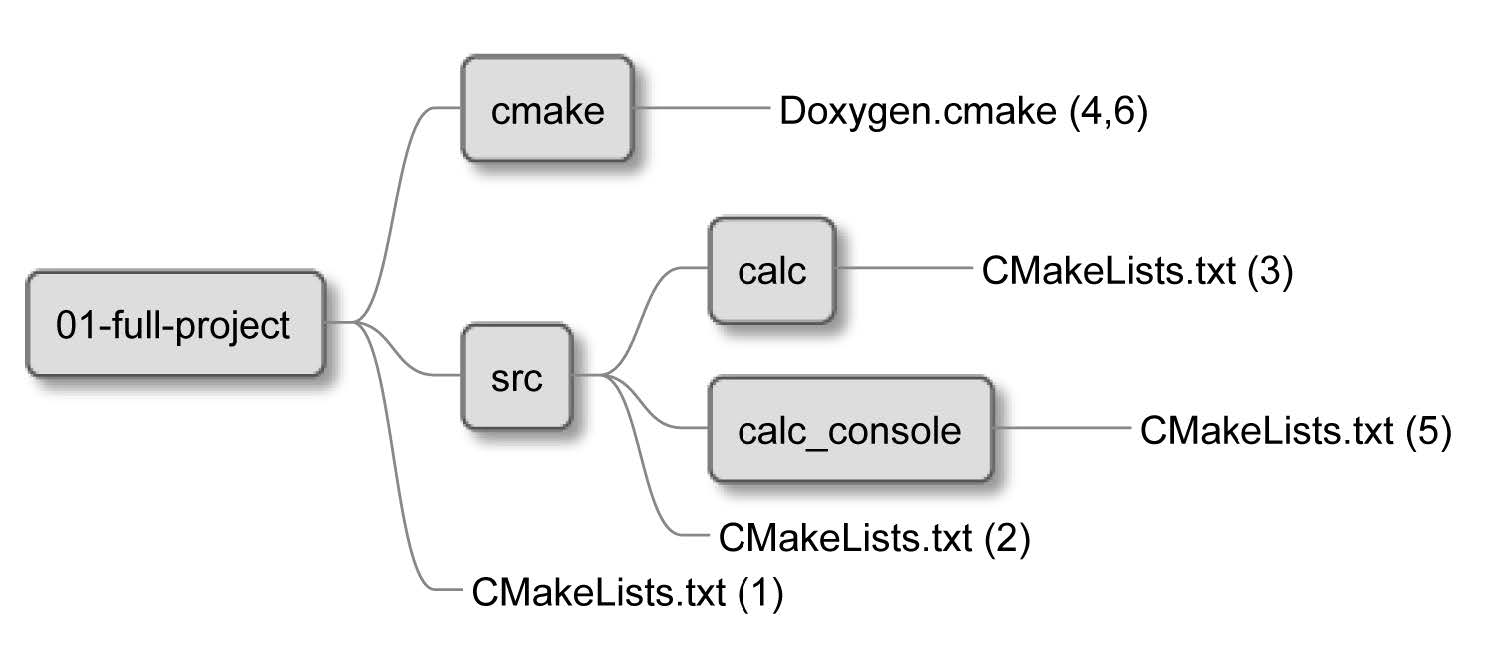
\includegraphics[width=0.8\textwidth]{content/3/chapter12/images/7.jpg}\\
Figure 12.7 – Files used to generate documentation
\end{center}

To generate documentation for our targets, we'll create another CMake utility module, Doxygen. We'll start by using the Doxygen find-module and downloading the doxygen-awesome-css project for themes:

\begin{lstlisting}[style=styleCMake]
# chapter-12/01-full-project/cmake/Doxygen.cmake (fragment)

find_package(Doxygen REQUIRED)
include(FetchContent)
FetchContent_Declare(doxygen-awesome-css
	GIT_REPOSITORY
		https://github.com/jothepro/doxygen-awesome-css.git
	GIT_TAG
		v1.6.0
)
FetchContent_MakeAvailable(doxygen-awesome-css)
\end{lstlisting}

Then, we'll need a function to create targets that generate documentation. We'll draw closely from code introduced in Chapter 10, Generating Documentation, and modify it to support many targets:

\begin{lstlisting}[style=styleCMake]
# chapter-12/01-full-project/cmake/Doxygen.cmake (continued)

function(Doxygen target input)
	set(NAME "doxygen-${target}")
	set(DOXYGEN_HTML_OUTPUT
		${PROJECT_BINARY_DIR}/${NAME})
	set(DOXYGEN_GENERATE_HTML YES)
	set(DOXYGEN_GENERATE_TREEVIEW YES)
	set(DOXYGEN_HAVE_DOT YES)
	set(DOXYGEN_DOT_IMAGE_FORMAT svg)
	set(DOXYGEN_DOT_TRANSPARENT YES)
	set(DOXYGEN_HTML_EXTRA_STYLESHEET
		${doxygen-awesome-css_SOURCE_DIR}/doxygenawesome.css)
	doxygen_add_docs(${NAME}
		${PROJECT_SOURCE_DIR}/${input}
			COMMENT "Generate HTML documentation"
	)
endfunction()
\end{lstlisting}

Now, we need to use this function by calling it for the library target:

\begin{lstlisting}[style=styleCMake]
# chapter-12/01-full-project/src/calc/CMakeLists.txt (continued)

# ... calc_static target definition
# ... testing and program analysis modules
include(Doxygen)
Doxygen(calc src/calc)
\end{lstlisting}

And we call it for the console executable:

\begin{lstlisting}[style=styleCMake]
# chapter-12/01-full-project/src/calc_console/CMakeLists.txt (continued)

# ... calc_static target definition
# ... testing and program analysis modules
include(Doxygen)
Doxygen(calc_console src/calc_console)

add_executable(calc_console bootstrap.cpp)
target_link_libraries(calc_console calc_console_static)
\end{lstlisting}

Two new targets are added to the project: doxygen-calc and doxygen-calc\_console, and technical documentation can be generated on demand.

What other documents should we provide?

\subsubsubsection{12.7.2\hspace{0.2cm}Not-so-technical documents of professional project}

Professional projects should always include at least two documents that are stored in a top-level directory:

\begin{itemize}
\item 
README – generally describes the project

\item 
LICENSE – specifies the legal characteristics of the project
\end{itemize}

You might also consider adding these:

\begin{itemize}
\item 
INSTALL – describes the steps required for installation

\item 
CHANGELOG – lists important changes that happened in different versions

\item 
AUTHORS – contains credits and contact information if a project has multiple contributors

\item 
BUGS – informs about known bugs and instructs how to report new ones
\end{itemize}

CMake as such doesn't play any role when it comes to these files – there's no automated behavior or scripts to use. However, these files are an essential part of C++ projects and should be covered for completeness. For reference, we'll provide a minimal set of exemplary files, starting with a short README file:

\begin{lstlisting}[style=stylePython]
# chapter-12/01-full-project/README.md

# Calc Console
Calc Console is a calculator that adds two numbers in a
terminal. It does all the math by using a **Calc** library.
This library is also available in this package.

This application is written in C++ and built with CMake.

## More information
- Installation instructions are in the INSTALL file
- License is in the LICENSE file
\end{lstlisting}

This is short and maybe a little silly. Note the .md extension – it stands for Markdown, which is a text-based formatting language that is easily readable. Websites such as GitHub and many text editors will render these files with rich formatting.

Our INSTALL file will look like this:

\begin{lstlisting}[style=stylePython]
# chapter-12/01-full-project/INSTALL

To install this software you'll need to provide the following:

- C++ compiler supporting C++17
- CMake >= 3.20
- GIT
- Doxygen + Graphviz
- CPPCheck
- Valgrind

This project also depends on GTest, GMock and FXTUI. This
software is automatically pulled from external repositories
during the installation.

To configure the project type:
cmake -B <temporary-directory>

Then you can build the project:
cmake --build <temporary-directory>

And finally install it:
cmake --install <temporary-directory>

To generate the documentation run:
cmake --build <temporary-directory> -t doxygen-calc
cmake --build <temporary-directory> -t doxygen-calc_console
\end{lstlisting}

This file turned out to be a bit longer, but it covers the most important requirements, steps, and commands, and it will work just fine for our needs.

The LICENSE file is a bit tricky, as it requires some expertise in copyright law (and otherwise). Instead of writing all clauses by ourselves, we can do what many other projects do and use a readily available software license. For this project, we'll go with the MIT License, which is extremely permissive. You might want to choose something else, depending on the needs of a specific project – check the Further reading section for some useful references:

\begin{lstlisting}[style=stylePython]
# chapter-12/01-full-project/LICENSE

Copyright 2022 Rafal Swidzinski

Permission is hereby granted, free of charge, to any person
obtaining a copy of this software and associated documentation
files (the "Software"), to deal in the Software without
restriction, including without limitation the rights to use,
copy, modify, merge, publish, distribute, sublicense, and/
or sell copies of the Software, and to permit persons to whom
the Software is furnished to do so, subject to the following
conditions:

The above copyright notice and this permission notice shall be
included in all copies or substantial portions of the Software.

THE SOFTWARE IS PROVIDED "AS IS", WITHOUT WARRANTY OF ANY
KIND, EXPRESS OR IMPLIED, INCLUDING BUT NOT LIMITED TO THE
WARRANTIES OF MERCHANTABILITY, FITNESS FOR A PARTICULAR PURPOSE
AND NONINFRINGEMENT. IN NO EVENT SHALL THE AUTHORS OR COPYRIGHT
HOLDERS BE LIABLE FOR ANY CLAIM, DAMAGES OR OTHER LIABILITY,
WHETHER IN AN ACTION OF CONTRACT, TORT OR OTHERWISE, ARISING
FROM, OUT OF OR IN CONNECTION WITH THE SOFTWARE OR THE USE OR
OTHER DEALINGS IN THE SOFTWARE.
\end{lstlisting}

Lastly, we have the CHANGELOG. As suggested earlier, it's good to keep track of changes in a file so that developers using your project can easily find out which version supports the features they need. For example, it might be useful to say that a multiplication feature was added to the library in version 0.8.2. Something as simple as the following is already helpful:

\begin{lstlisting}[style=stylePython]
# chapter-12/01-full-project/CHANGELOG

1.0.0 Public version with installer
0.8.2 Multiplication added to the Calc Library
0.5.1 Introducing the Calc Console application
0.2.0 Basic Calc library with Sum function
\end{lstlisting}

Our professional project is now complete – we can build it, test it, generate packages, upload all sources to a repository, and release artifacts. Of course, it would be easier if this could happen automatically, perhaps with a CI/CD pipeline. But that's a story for another book.












